 %Linea Para poder completar automaticamente las citas con el Sublime
%No hace el documento, se puede borrar esta linea si no se usa el Sublime
%------------------------------------------------------------------------------
 \newcommand{\NoBiblioIntro}[1]{
 \ifthenelse{\equal{#1}{verdadero}}{}{\bibliography{Referencias/base_bibliografica}}
 \NoBiblioIntro{verdadero}}
 %-----------------------------------------------------------------------------

%Formato (Nombre de capitulo largo o corto), nombre del capitulo y estilo de la
%Portada del Capitulo
%------------------------------------------------------------------------------

 %Formato en si, titulo en un solo renglon
 \FormatoCapituloUnaLinea

 %Nombre y etiquete para referir
 \chapter{Introducción}\label{chap:Introduccion}
 %\label{chap:Introduccion}

 %Para que no salga el numero de pagina en la portada del capitulo
 \thispagestyle{empty}
	
 %Resumen del Capitulo en Italica
 %\noindent\textit{El propósito de este capítulo es introducir los temas que se tratarán en la tesis y hacer una breve reseña de los  aspectos teórico de las técnicas y procesos que se utilizaron a la largo de la tesis. Al final se enumerna las motivaciones y objetivos del presente trabajo.}

 
 %Indice de capitulo alineada al borde inferior de la pagina, nueva pagina
 \vfill
 \minitoc
 \newpage
 %-------------------------------------------------------------------------------

\section{Breve reseña sobre nanotecnología}

	 El 29 de diciembre de 1959, en una conferencia titulada \textit{<<There's Plenty of Room at the Bottom>>}, el físico Richard Feynman, considerado por muchos el padre de la nanotecnología, sugirió que se podría escribir toda la Enciclopedia \textit{Britannica} en la cabeza de un alfiler.\cite{Feynman1959} Esta presentación fue sin duda más conceptual e inspiradora que estrictamente científica, anterior al uso masivo de las técnicas de microscopía electrónica y al desarrollo de las microscopías de efecto túnel y fuerza atómica.  

	 Algunos años más tarde, en 1974, Taniguchi incorporó por primera vez el término nanotecnología para describir procesos de microfabricación como depósito de películas delgadas o \textit{ion millling} y lo definió como <<aquellos procesos de separación, consolidación y deformación de los materiales átomo por átomo o molécula por molécula>>. \cite{taniguchi1974} Fue Drexler quién finalmente popularizó el término en su libro \textit{<<Engines of Creation: The Coming Era of Nanotechnology>>}\cite{drexler1987}. 

	 Una definición más actual y consensuada para nanotecnología es la presentada por la \textit{National Nanotechnology Initiative} (NNI, \url{http://nano.gov/nanotech-101/what/definition}): desarrollo tecnológico de estructuras y sistemas en una escala nanométrica, entre 1 y \SI{100}{\nm}. Se podría, también, establecer una definición funcional: uso e implementación tecnológica de nanociencia. Esta rama de la ciencia se caracteriza fundamentalmente por ser multidisciplinaria y abarcar muchas áreas del conocimiento, ciencia de materiales, química, física y biología (por citar algunas), las cuales interactúan entre sí para generar un espacio sinérgico entre ellas. Cuando los descubrimientos en nanociencia son potencialmente aplicables a productos interviene la nanotecnología, tendiendo un lazo entre la ciencia y la industria para llevar a cabo desarrollos tecnológicos o escalar prototipos que eventualmente puedan acabar en productos de consumo.
	
	 Al\space realizar una búsqueda en la base de datos Scopus\textsuperscript\textregistered (\url{http://www.scopus.com}) de las publicaciones que contienen las palabras en inglés para nanotecnología (\textit{nanotechnology}), nanofísica (\textit{nanophysics}), nanoquímica (\textit{nanochemistry}), nanoescala (\textit{nanoscale}) y nanociencia (\textit{nanoscience}) se obtienen los resultados de la figura \ref{fig:publicaciones-ano}. 

	 Del análisis de dicho gráfico se observa que las publicaciones que contiene la palabra nanotecnología en el título, resumen o como palabra clave son mucho mayor que las que contiene nanoescala, nanociencia, nanofísica o nanoquímica. Contrariamente a la evolución histórica de las ``ciencia aplicadas'', donde primero es el descubrimiento científico y luego el desarrollo tecnológico, la nanotecnología parece presentarse como impulsora, no solo de desarrollos tecnológicos sino también como impulsora de ``ciencias básicas''.

	 Whitesides y Deutch en su artículo \textit{<<Let's get practical>>}\cite{Burdass2010} opinan que la química, como rama de la ciencia básica y como industria madura, debe reinventarse para acondicionarse a los requerimientos de la sociedad actual y poder seguir respondiendo preguntas fundamentales a la vez que resuelve problemas de índole práctica. Los autores afirman que los ``problemas prácticos'' son generalmente despreciados por las ciencias básicas.  Sin embargo éste no parece ser un problema de la nanotecnología, la cual ha hecho grandes contribuciones al desarrollo científico a pesar de ser una disciplina que en general busca resolver problemas prácticos.
			

	 \pagebreak Este hecho se ve reflejado al agrupar los resultados de la búsqueda por países (figura \ref{fig:publicaciones-ano}), dónde vemos que aquellos que más publicaciones tienen con la palabra nanotecnología son, como es de esperar, los países más desarrollados tecnológicamente ocupando los primeros cinco lugares Estados Unidos, China, Japón, Alemania y Reino Unido. En América Latina, el primero es Brasil con 1453 publicaciones seguido de Argentina con 567 (figura \ref{fig:paises}).


 			\begin{figure}[h!]
 			\begin{center}
 			\hspace{0.3cm}\includegraphics[width=0.85\textwidth]{Graficos/busqueda-por-ano.pdf}
 			\vspace*{-0.6cm}
 			\caption[Publicaciones por año en nanotecnología]{Publicaciones científicas por año que contienen la palabra \textit{nanotechnology}, \textit{nanoscale}, \textit{nanoscience}, \textit{nanochemistry} o \textit{nanophysics} en el título, resumen o palabras claves.}
 			\label{fig:publicaciones-ano}
 			\vspace*{-0.2cm} 		    
 			\end{center}
 		    \end{figure}

			\begin{figure}[b!]
 				\begin{center}
 				\includegraphics[angle=270,width=0.92\textwidth]{Graficos/histogramas-ciencia.pdf}
 				\vspace*{-0.4cm}
 				\caption[Nanotecnología por países]{Distribución por países del número de publicaciones científicas con la palabra nanotecnología. Datos obtenidos de la base de datos Scopus\textsuperscript\textregistered.}
 				\label{fig:paises}
 		    	\end{center}
 		    	\end{figure}

	 Además de producción científica y desarrollos tecnológicos, la nanotecnología cuenta con patentes internacionales y productos industriales de consumo masivo en el mercado global. Existen bases de datos que registran la actividad del sector creando informes sobre estos productos, patentes, estándares y compañías de base nanotecnológica. Podemos mencionar algunas de ellas como el \textit{Nanotechnology Consumer Products Inventory} (CPI) (\url{http://www.nanotechproject.org/cpi/}) creada por \textit{The Project on Emerging Nanotechnologies} en 2005\cite{Vance2015}; la \textit{Nanotechnology Products Database} (NPD) (\url{http://http://product.statnano.com/}) creada con apoyo del \textit{Iran Nanotechnology Initiative Council} (INIC) en 2010 y \textit{The Nanodatabase} (\url{http://nanodb.dk}), iniciativa desarrollada por \textit{DTU Environment, Danish Ecological Council} y \textit{Danish Consumer Council} en 2011. En el gráfico de la figura \ref{fig:productos} se resumen algunos datos registrados en cada una de ellas, agrupados por cantidad productos con base nanotecnológica, número de empresas que los generan y cantidad países donde se encuentran distribuidas.

		\begin{figure}[ht!]
 			\begin{center}
 			\includegraphics[angle=270,width=0.92\textwidth]{Graficos/productos2.pdf}
 			\caption[Cantidad de productos, compañías y origen con base nanotecnologica]{Registros de empresas y países generadores de productos que incorporan nanotecnología. Extraído de las bases de datos \textit{Nanotechnology Consumer Products Inventory} (CPI), \textit{Nanotechnology Products Database} (NPD) y \textit{The Nanodatabase}.}
 			\label{fig:productos}
 		    \end{center}
 		    \end{figure}

 	 También existen numerosas patentes que registran productos con nanotecnología. En la figura \ref{fig:patentes} se muestra la evolución desde el año 2001 hasta el 2016 del número de patentes registradas por la \textit{European Patent Office} (EPO) y por la \textit{United States Patent and Trademark Office} (USPTO).

     Muchos de estos productos pertenecen al rubro alimenticio y cosmético. Nanopartículas de Ag, TiO$_2$ o SiO$_2$ se incorporan en los alimentos o en los envases como conservantes, agentes antimicrobianos, colorantes y antioxidantes. En la industria cosmética el mayor uso de los nanomateriales es para dar color, textura y como filtros solares.
 	
 	 La inclusión de nanomateriales en el mercado, especialmente en estos dos rubros, obliga la incorporación de recomendaciones, estandarización y regulaciones en el campo de la nanotecnología. El\hspace{1pt} documento\hspace{1pt} CEN/TC\hspace{1pt} 352 de abril de 2016 \url{https://standards.cen.eu/dyn/www/f?p=204:7:0::::FSP_ORG_ID:508478&cs=1A6FDA13EC1F6859FD3F63B18B98492ED})
 	 del \textit{European committee for Standardization}(CEN), ofrece guías para la identificación, detección y cuantificación de nano-objetos en matrices complejas. La \textit{International Organization for Standardization} (ISO) creó en 2005 una serie de documentos ISO/TC 223 (\url{https://www.iso.org/committee/381983.html}) con el objetivo de definir y establecer el alcance de las nanotecnologías. Define allí una serie de parámetros y descriptores para caracterizar e identificar nanopartículas, tamaño, forma, distribución, composición química, carga superficial, estado de agregación, solubilidad y área especifica entre otros.

 	 Este contexto de regulaciones emergentes en el campo de la nanotectnología obliga a los institutos metrológicos de los distintos países (entre ellos el INTI, como Instituto Metrológico Nacional) a generar nanomateriales de referencia y validar las técnicas y procedimientos para su detección y cuantificación.

 	 Hasta el momento se ha hecho una breve introducción sobre la historia y situación actual de la nanotecnología, pero ¿como se construyen los nanomateriales?.


		\begin{figure}[h!]
 			\begin{center}
 			\includegraphics[width=0.92\textwidth]{Graficos/patentes.pdf}
 			\vspace*{-0.3cm}
 			\caption[Número de patentes de productos en base nanotecnológica]{Número de patentes registradas por año en la oficinas de patentes de los Estados Unidos y Europa. Datos extraídos de \url{http://statnano.com/}.}
 			\label{fig:patentes}
 		    \end{center}
 		    \end{figure}

 	\vspace*{-0.6cm}\subsection{Síntesis de nanomateriales y construcción de nanoestructuras}

		Existen dos enfoques posibles para obtener estructuras y objetos en la nanoescala. El primero se trata de realizar estructuras por grabado, maquinado o molienda de un material, para reducirlo a dimensiones nano en un proceso de miniaturización. Esta aproximación se denomina ``de arriba hacia abajo'' o más conocida como \textit{top-down}. La electrónica actual de consumo masivo (incluyendo computadoras y dispositivos móviles) se basa en esta aproximación. El segundo enfoque es aquel denominado de ``abajo hacía arriba'' o \textit{bottom-up}, el cual consiste en la construcción de objetos a partir de bloques fundamentales, los cuales pueden ser átomos o moléculas. 

		La nanotecnología se caracteriza por aprovechar propiedades diferenciales que surgen en esta escala. La mayoría de estos cambios en las propiedades ópticas, eléctricas, magnéticas o mecánicas se descubrieron procesando materiales mediante el enfoque \textit{bottom-up}, impulsando nuevas formas de sintetizar materiales, p. ej. grafeno, nanotubos de carbono o fullerenos. Faraday fue uno de los primeros científicos en sugerir que, en la escala nanométrica, el cambio en las propiedades de la materia está ligado al tamaño, estudiando el cambio de color en coloides de Au\cite{faraday1857}. A este grupo pertenecen las técnicas químicas de síntesis de nanopartículas, nanobarras y películas delgadas, métodos de autoensamblado y química supramolecular; también técnicas de crecimiento en fase vapor: epitaxial, \textit{physical vapour deposition (PVD)}, \textit{chemical vapour deposition} (CVD) y \textit{atomic layer deposition (ALD)}.
			
		Es de esperar que la verdadera revolución nanotecnológica dé un salto de calidad cuando converjan ambos enfoques, aprovechando las ventajas que ofrece cada uno de ellos. Este se trata de un enfoque ``funcional'', en el cual lo importante es el objetivo, ya sea un trabajo científico, prototipo o un producto.

		Soler-Illia expone en su libro <<Nanotecnología: el desafío del siglo XXI>>\cite{nanotecnologia-galo} que es en éste período de la historia donde se esta llevando a cabo esta convergencia. A modo de ejemplo presentan un gráfico esquemático donde muestra la evolución de ambos enfoques hacia la convergencia en la nanoescala.

			\begin{figure}[ht!]
 				\begin{center}
 				\includegraphics[width=0.95\textwidth]{Imagenes/convergencia2.png}
 				\caption[Convergencia \textit{top-down }y \textit{bottom-up.}]{Convergencia temporal de las aproximaciones \textit{top-down }y \textit{bottom-up.} Figura extraída de <<Nanotecnología: El desafío del siglo XXI>>.\cite{nanotecnologia-galo}}
 				\label{fig:galo-convergencia}
 		   	    \end{center}
 		   	    \end{figure}

    	Esta tesis tiene por objetivo fabricar multisensores utilizando electroquímica como herramienta analítica de detección. La fabricación de los multisensores se realiza en base a procesos \textit{top-down} para escalar y miniaturizar los electrodos y procesos \textit{bottom-up} (química sol-gel y autoensamblado inducido por evaporación) con el fin sintetizar la película activa. El diagrama de  de Venn de la figura \ref{fig:sensores} muestran los elementos necesarios para la fabricación de los sensores electroquímicos basados en películas delgadas mesoporosas. 
	 	
 		En las siguientes secciones se tratan brevemente los fundamentos teóricos de cada una de las áreas temáticas exploradas para el desarrollo de la plataforma de sensores electroquímicos en base a películas delgadas mesoporosas y hacía el final del capítulo se exponen los objetivos y motivaciones que llevaron a materializar esta tesis.


	       \begin{figure}[ht!]
 				\begin{center}
 				\includegraphics[width=0.65\textwidth]{Esquemas/concepto-interdiplinario.pdf}
 				\caption[Plataforma de sensores. Diagrama de Venn.]{Elementos necesarios para el desarrollo y fabricación de la plataforma de sensores electroquímicos basados en películas delgadas mesoporosas.}
 		   		\label{fig:sensores}
 		    	\end{center}
 		    	\end{figure}

\section{Películas delgadas mesoporosas}\label{sec:mesoporosos}
	
	 El término película delgada o lámina delgada hace referencia a una capa de material cuyo espesor va desde unos pocos manómetros a algunos micrones, típicamente entre 10 y \SI{1000}{\nm}. El control en el espesor de la película es una etapa fundamental para cualquier aplicación, más aun cuando se trata de controlar la propiedades que surgen debido a la dimensión nanométrica en el espesor (p. ej. fenómenos de interferencia de luz en el rango visible con espesores de unos cientos de nanómetros). 

     Las películas delgadas son elaboradas a partir de técnicas químicas que utilizan precursores moleculares, típicamente mediante \textit{bottom-up}. Dentro de ellos se pueden nombrar los procesos de autoensamblado molecular, electrodeposición, crecimiento epitaxial, técnicas de deposición químicas o físicas en fase vapor, sol-gel y autoensamblado inducido por evaporación entre las más populares. En particular las películas delgadas mesoporosas (\pdm) son aquellas que además de la característica de ser delgadas, son porosas, con arreglos de poros ordenados a largo o corto alcance.

	 La \textit{International Union of Pure and Applied Chemistry} (IUPAC) definen los materiales mesoporosos como aquellos que presentan poros monodispersos entre 2 y \SI{50}{\nm}. La Real Academia Española tiene tres acepciones para la palabra <<poro>>. Dos se ellas son <<Espacio que hay entre las moléculas de los cuerpos>> e <<Intersticio que hay entre las partículas de los sólidos de estructura discontinua>> (\url{http://dle.rae.es/?id=ThdH0Y9%7CThe6N27%7CThgVys6}). Según esta definición todos los materiales presentan poros (excepto por supuesto los átomos o moléculas individuales, pero estos no entran dentro de la definición de material), resulta entonces, indispensable cuantificar la porosidad o la cantidad de poros en un material.\cite{Brinker1990,Lu1997,Innocenzi2013}

	 \pagebreak La porosidad es una medida de los espacios vacíos (poros) en un material y se define como la fracción del volumen de poros sobre el volumen total, entre 0 y 1 (o entre 0\% y 100\%).\cite{iupac-1994} Confiere a los materiales importantes propiedades, como una baja densidad, lo que supone un peso ligero y gran área superficial para almacenar moléculas en los poros. Además, el tamaño del poro puede funcionar como un tamiz para separar moléculas de distintos tamaños.\cite{Martin2004} 

	\subsection{Síntesis de óxidos mesoporosos} 

	 La producción de óxidos mesoporosos (ya sean polvos, películas o xerogeles) se realiza a través de la combinación de precursores inorgánicos y tensioactivos, que actúan como agentes porógenos. Involucra dos procesos concertados: la formación y el autoensamblado de micelas, molde de la estructura de poros, y las reacciones químicas de hidrólisis y condensación del precursor inorgánico que formará el óxido. 

				\begin{figure}[h!]
 				\begin{center}
 				\includegraphics[width=\textwidth]{Esquemas/oxido-meso.pdf}
 				\caption[Esquema general para la formación de un óxido mesoestructurado]{Esquema general para la formación de un óxido mesoporoso combinando precursores inorgánicos y tensioactivos para la moldear los poros.}
 		   		\label{fig:oxmeso}
 		    	\end{center}
 		    	\end{figure}

	 En la Figura \ref{fig:oxmeso} se muestra un esquema de los pasos involucrados en la obtención de óxidos mesoporosos. En una primera etapa se forma un sistema híbrido orgánico-inorgánico que contiene al surfactante rodeado por el óxido (sistema mesoestructurado). En un segundo paso, se elimina el surfactante dando lugar a la estructura porosa. La eliminación del surfactante puede ser por calcinación o extracción.
 

     El primer antecedente de una síntesis de sílice mesoporosa se registra en una patente del año 1971. Sin embargo, el campo de los materiales mesoporosos comenzó a desarrollarse de manera explosiva a partir del trabajo del grupo de Mobil. Científicos de esta firma reportaron en 1992 la síntesis en polvo de la familia de sílices mesoporosas conocida como M41S (MCM-41, MCM-48, etc.).\cite{Kresge1992,Beck1992} Entre 1997 y 1998 se reportaron los primeros trabajos en los cuales se obtuvieron óxidos de silicio mesoporoso en forma de película delgada mediante técnicas de evaporación controlada y \textit{dip-coating}.\cite{Lu1997,Zhao1998a,Zhao1998,Brinker1999} 

     A partir de estos trabajos pioneros, el número de publicaciones sobre potenciales aplicaciones y usos creció considerablemente, reportándose síntesis para óxidos de metales de transición \cite{Ciesla1996,Ulagappan1996,Antonelli1995}, óxidos híbridos, poros de una gran variedad de tamaños, estructuras porosas jerárquicas, etc.\cite{Soler-Illia2006,Moller1998} %CITAS
   
	\subsection{Química sol-gel}

	 Los procesos tipo sol-gel refieren a una síntesis inorgánica en la cual se parte de un precursor molecular. Mediante reacciones de hidrólisis y de condensación evoluciona en una dispersión coloidal (sol) hasta la formación de una estructura inorgánica tipo gel o densa del material deseado. Dependiendo del procesamiento del sol, se pueden obtener distintas formas de la materia según las aplicaciones o los usos para los cuales se quieran emplear los productos de la síntesis. Entre ellas se cuentan: fibras, nanopartículas, polvos, películas delgadas densas o porosas, aerogeles y xerogeles por citar los más utilizados. La figura \ref{fig:sol-gel-process} ilustra algunos de estos procesos.

	 		\begin{figure}[ht!]
 				\begin{center}
 				\includegraphics[width=\textwidth]{Esquemas/sol-gel.pdf}
 				\caption{Algunas de las posibles formas de procesar un material obtenido mediante química sol-gel. Adaptado de \textit{<<Sol Gel Science. The Physics and Chemistry of Sol Gel Processing>>}.\cite{Brinker1990}}
 				\label{fig:sol-gel-process}
 		   	    \end{center}
 		   	    \end{figure}

	 El control sobre la cinética de tales reacciones permite disponer de formas y estructuras diferentes, tanto en cuanto a la cristalinidad como a la porosidad del cerámico resultante. Las temperaturas involucradas en la fabricación de materiales cerámicos mediante síntesis sol-gel son muy inferiores ($\leq$\SI{400}{\celsius}) a aquellas empleados por  los métodos tradicionales ($\geq$\SI{700}{\celsius}).\cite{Brinker1990,Jolivet2000,Wright2001}

	 La formación de un óxido por el método sol-gel implica conectar centros metálicos mediante puentes oxo o hidroxo para generar (hidroxo)polímeros de metal en solución. Para ello se hace reaccionar un precursor MX$_4$ con agua, donde M es el elemento del cual se quiere obtener el óxido, y X es un grupo saliente como por ejemplo un anión inorgánico o un grupo –OR. El primer paso de la reacción es la hidrólisis de un grupo alcóxido (o de un anión) para dar lugar a un hidroxocompuesto, tal como se ejemplifica en la ecuación \ref{eq:hidrosg1} para el caso de un alcóxido.
			
			 \begin{equation}
 				\begin{aligned}
 				\includegraphics[scale=0.70]{Esquemas/sg1.pdf}
 				\end{aligned}
 				\label{eq:hidrosg1}
 	 			\end{equation}

    	Luego, la especie hidroxilada puede reaccionar con otros centros metálicos, dando lugar a reacciones de condensación, cuyos productos son oligómeros que eventualmente evoluciona en partículas de óxido. La condensación puede dar lugar a un puente oxo, tal como se muestra en la ecuación \ref{eq:oxosg2} (oxolación) o un puente hidroxo, tal como se observa en \ref{eq:olasg3} (olación). 

			\begin{equation}
		    	\begin{aligned}
 	 	 		\includegraphics[width=0.9\textwidth]{Esquemas/sg2.pdf}
 	 	 		\end{aligned}
 	 	 		\label{eq:oxosg2}
 	 	 		\end{equation}

			\begin{equation}
 	 	 		\begin{aligned}
 	 	 		\includegraphics[width=0.9\textwidth]{Esquemas/sg3.pdf}
 	 	 		\label{eq:olasg3}
 	 	 		\end{aligned}
 	 	 		\end{equation}

	 Las etapas de hidrólisis y condensación son análogos a la activación y la propagación en la polimerización orgánica, por lo que el proceso sol-gel puede calificarse como una polimerización inorgánica controlada. Un manejo adecuado de las variables (concentración de precursores, catalizadores, pH, solvente) y condiciones de síntesis (temperatura, humedad, tiempos de cada etapa de reacción) lleva a sistemas donde se pueden controlar con precisión  la estructura inorgánica, la porosidad, la incorporación de funciones orgánicas, la relación de composiciones en óxidos mixtos (MM') y otras características del sistema.

	 Uno de los pilares de este trabajo fue utilizar óxidos mesoporosos procesados en forma de películas delgadas para obtener membranas permeoselectivas. Para este fin el sol se depositó sobre distintos sustratos y fue fundamental controlar las variables de síntesis antes citadas, ya que definen las características finales de los óxidos, que a su vez establecieron las propiedades permeoselectivas de las películas delgadas mesoporosas.

	 Para profundizar sobre estos temas se recomienda la lectura de los libros \textit{Sol Gel Science. The Physics and Chemistry of Sol Gel Processing}\cite{Wright2001} o \textit{Introduction to Sol Gel Processing.} \cite{Pierre1998} 
	
	\subsection{Autoensamblado inducido por evaporación (AEIE)}

	 El proceso de autoensamblado inducido por evaporación (AEIE) fue introducido por el grupo de Brinker a fines de la década de 1990.\cite{Lu1997,Brinker1999} Consiste en la formación de estructuras supramoleculares híbridas orgánicas\textbar inorgánicas con organización en la nanoescala. Dichas estructuras son obtenidas mediante la evaporación del solvente en soluciones que contiene al precursor inorgánico, agentes de control para la hidrólisis y condensación y un agente porógeno, el tensioactivo que inicialmente se halla disuelto. Este proceso ocurre cooperativamente con la interacción y condensación de los precursores inorgánicos. En la actualidad, este concepto constituye un método habitual de obtención de \pdm\space ordenadas\cite{Grosso2004} así como micropartículas, monolitos, aerosoles, etc.\cite{Yang1998a}


	 Existen muchas técnicas de depósito de \pdm. Las más utilizadas son \textit{spin-coating}, \textit{dip-coating} y \textit{spray-coating}. En la figura \ref{fig:autoensam} se ejemplifica el proceso de AEIE cuando se aplica la técnica de \textit{dip-coating}. Allí se destacan los principales eventos que ocurren al retirar el sustrato de la solución a velocidad controlada. El sol, en términos generales, está compuesto por un solvente volátil, precursores inorgánicos, agua y el surfactante deseado. A medida que se retira el sustrato, se evapora el solvente y consecuentemente se concentra el surfactante mas allá de la concentración micelar crítica (cmc), formando micelas, que luego se organizarán en un cristal líquido. La estructura de dicho cristal impacta directamente en la estructura final de las \pdm. Procesos similares ocurren cuando se obtienen \pdm\space por \textit{spin-coating}. 
 				
   	 En función de la composición inicial del sol, del tipo de surfactante, de la química de los precursores, del sustrato, de las parámetros de depósito y de las condiciones ambientales es posible obtener diferentes entornos que darán lugar a distintos arreglos tridimensionales de poros, que está dado por el organización micelar previa al momento en el cual se elimina el surfactante ya sea por calcinación o extracción.\cite{Grosso2004,Grosso2002,Crepaldi2002a,Grosso2003,Violi2015} 
		

	 	\begin{figure}[h!]
 				\begin{center}
 				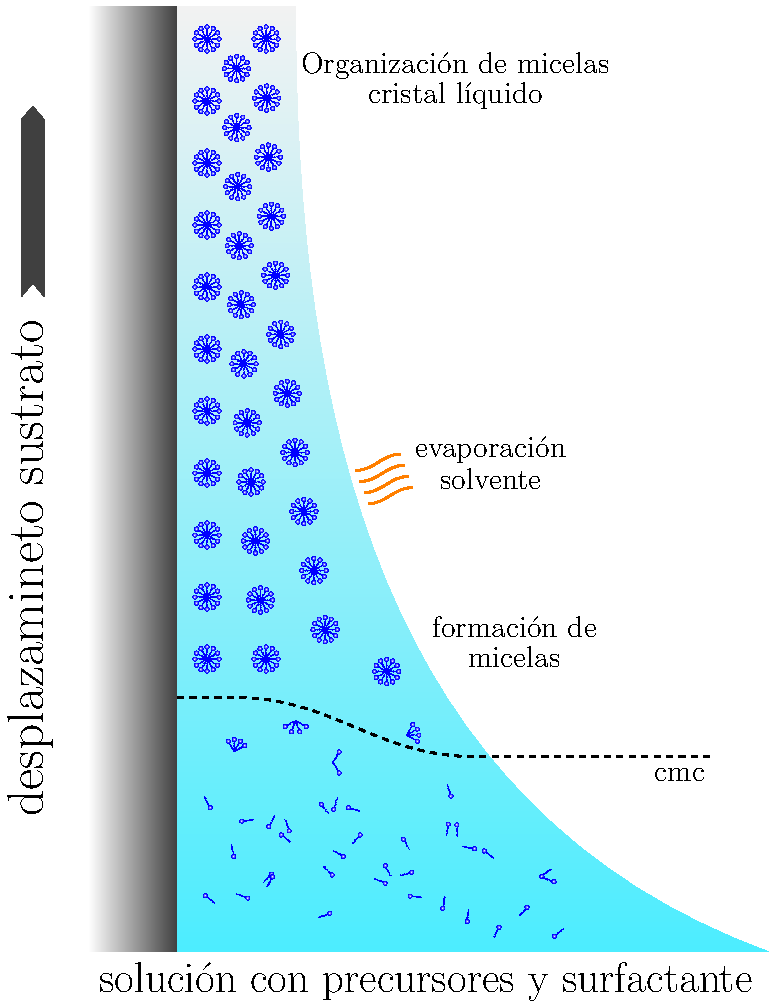
\includegraphics[width=0.5\textwidth]{Esquemas/autoensam.pdf}
 				\caption[Proceso de autoensamblado inducido por evaporación (AEIE)]{Proceso de autoensamblado inducido por evaporación (AEIE) mediante \textit{dip-coating.} La evaporación del solvente favorece la formación de micelas mas allá de la cmc formado el cristal líquido. Un proceso similar ocurre cuando se aplica la técnica de \textit{spin-coating.} Adaptado de <<Films delgados mesoporosos de óxidos metálicos, mixtos e híbridos. Hacia un diseño racional de nanomateriales funcionales>>\cite{Angelome2008}.}
 		   		\label{fig:autoensam}
 		    	\end{center}
 		    	\end{figure}

\section{Técnicas electroquímicas}
					
		Existen muchas técnicas electroquímicas basadas en mediciones de potencial, corriente, impedancia o conductividad.\cite{Wi2000,Bockris1974,koryta1993}

		Una de las más difundidas y utilizadas es la voltametría. Ésta técnica se aceleró con las investigaciones sobre polarografía en 1922 por el Premio Nobel de Química Jaroslav Heyrovský.\cite{Zuman1960} En 1942, Hickling construyó el primer potenciostato de tres electrodos, configuración típica de cualquier experimento que involucre una voltametría. \cite{hickling1942} Durante las décadas del 60 y 70 se hicieron muchos avances en la teoría, la instrumentación y la introducción de sistemas automatizados controlados por computadoras. Estos avances mejoraron la sensibilidad y crearon nuevos métodos analíticos. La industria respondió con la producción de potenciostatos más económicos y diversificados, electrodos de trabajo específicos, electrodos de referencia y celdas utilizadas eficazmente en el trabajo analítico de rutina.\cite{Wi2000}

		Un experimento voltamperométrico se fundamenta en medir la corriente que genera una especie electroactiva entre dos electrodos en función de la variación del potencial aplicado sobre un electrodo, denominado electrodo de trabajo. La diferencia de potencial se establece contra un potencial de referencia fijo, el electrodo de referencia. El resultado es un gráfico de corriente versus potencial denominado voltagrama.

		La interpretación de los voltagramas y el análisis de datos requiere de consideraciones cinéticas, además de termodinámicas, debido al componente temporal de la voltametría. Relaciones teóricas desarrolladas en los últimos años del siglo XIX, tales como la ecuación de Nernst, consideran sistemas electroquímicos en equilibrio termodinámico y están expresadas independientemente de la componente temporal, por lo tanto son insuficientes por sí mismas para describir los aspectos dinámicos de la voltametría.\cite{nnnicholson1964}

		En 1930 Butler y Volmer publican un artículo en el cual desarrollan un expresión conocida como la ecuación de Butler-Volmer (ec. \ref{eq:butler}), una de las más importantes en cinética electroquímica, cuya expresión más general es\cite{Erdey-Gruz1930}: 

			\vspace*{3mm}
			\begin{equation}
			j=j_0\left[\exp\left(\frac{\alpha_azF}{RT}(E-E_{eq})\right)-\exp\left(-\frac{\alpha_czF}{RT}(E-E_{eq})\right)\right]
			\label{eq:butler}
			\end{equation}
			\vspace*{3mm}

		\noindent esta ecuación describe cómo evoluciona la corriente en un electrodo dependiendo del potencial del mismo, considerando tanto la reacción de reducción como la de oxidación, donde $j$ es la densidad de corriente, $j_0$ la corriente de intercambio, $E$ el potencial del electrodo de trabajo, $E_{eq}$ el potencial de equilibrio, $z$ el número de electrones involucrados y $\alpha_c$ y $\alpha_a$ son coeficiente de transferencia de carga catódico y anódico respectivamente. A partir de consideraciones de casos límites para esta expresión y de simulaciones por computadora se pueden explicar numerosas respuestas electroquímicas.

		Existen muchos tipos de voltametrías tales como: voltametría cíclica, de barrido lineal, escalonada, de onda cuadrada, de corriente alterna, etc. En la sección \ref{sec:medidas_eq} se amplía la información sobre algunos aspectos de las variantes voltamperométricas usadas en esta tesis y se describen cuidadosamente las variables experimentales empleadas. \textit{Electrochemical Methods: Fundamentals and Applications}\cite{Wi2000} y  \textit{Principles of electrochemistry}\cite{koryta1993} son dos excelentes tratados sobre electroquímica en los cuales se pude profundizar el tema ampliamente, tanto en aspectos teóricos como experimentales. 

		Comercialmente se producen un gran número de sistemas voltamperométricos para la determinación de determinadas especies que son de interés en la industria y la investigación. Estos dispositivos se denominan a veces electrodos, pero son, de hecho, celdas electroquímicas completas y son más conocidas como sensores amperométricos. Muchos de ellos son para detección de O$_2$, gases tóxicos, glucosa y una gran variedad de analitos tanto orgánicos como inorgánicos. Estos ofrecen ventajas importantes en el análisis multicomponente, entre ellas alta selectividad y sensibilidad, alta relación señal-ruido, bajo límite de detección y miniaturización.\cite{bakker2006,stradiotto2003,harris2013,Ciosek2007,Kojima2003}
			
\section{Miniaturización y escalabilidad}\label{sec:microfabricacion}\label{sec:intro_fotolito}
		
		Como se mencionó anteriormente, las técnicas para fabricar electrónica de consumo masivo rentable, a gran escala y de pequeñas dimensiones son las conocidas como <<técnicas de microfabricación>>, basadas en la aproximación \textit{top-down}. \cite{Jaeger2001}

		En el año 1947, los físicos Bardeen, Brattain y Shockley de la compañía \textit{Bell Telephone Company}, publicaron la fabricación del primer transistor. Dicho invento fue la piedra fundamental de la revolución electrónica de las últimas cinco décadas. Fabricado con germanio y de unos \SI{7}{cm} de alto estaba muy lejos de convertirse en la unidad básica del cálculo computacional que es hoy en día. \cite{riordan1999} 

		Años más tarde, en 1957, ocho hombres dejaron de trabajar en \textit{Shockley Semiconductor Laboratory} para formar la compañía \textit{Fairchild Semiconductor}. A este grupo de personas se los conoce como los ``niños de Fairchild''. Entre sus miembros se destacaron: Hoerni, quién patentó, en 1959, el primer proceso de fabricación planar basado en   procesos difusivos de impurezas sobre discos de silicio monocristalinos; Noyce quién junto con Kilby son considerados como los inventores de los circuitos integrados o \textit{microchip}; y Moore, cofundador de \textit{Intel Corporation}, quién publicó un documento en 1965, conocido como Ley de Moore, en el cuál anticipaba que cada año se duplicaría el número de transistores en un microprocesador. En 1975 el propio Moore reformularía su ley extendiendo el período a 24 meses en lugar de 12. \cite{moore2006,riordan1999,fagen1984}

		A partir de estos hitos tecnológicos la industria de los semiconductores se convirtió en una de las grande a nivel mundial, siendo hoy en día es una industria madura, de enormes proporciones y de las más rentables del mundo, productora de computadoras, celulares, tabletas, acelerómetros, giroscópos, sistemas de posicionamiento global, etc. Dicha industria se puede dividir en dos grandes grupos: en la industria de los micro/nano sistemas eléctrico mecánicos (MEMS/NEMS, del inglés \textit{Micro/Nano Electric Mechanicals Systems}) o en la de los circuitos integrados (IC, del inglés \textit{integrated circuit}). Al\space primer grupo pertenecen dispositivos como sensores, actuadores y controladores y al segundo grupo los microprocesadores y memorias que se basan casi exclusivamente en una unidad mínima de procesamiento compuesta por transistores.\cite{Franssila2004,Jaeger2001,Madou2002}

 		Mediada la década de los 90 la industria de los semiconductores se sumerge en la nanotecnología, no por las nuevas propiedades que pueden surgir, sino por la necesidad de integración y de hacer dispositivos más densos, con mayor cantidad de componentes por unidad de área. La miniaturización permite obtener dispositivos cada vez más  veloces, que funcionan a mayores frecuencias, con menor disipación de potencia y a un menor costo. Todos estos requerimientos o necesidades tecnológicas se fueron materializando en un mercado de un capital enorme, que a su vez, se nutre de la industria, la cual se basa en la evolución de las técnicas y procesos de microfabricación.

	\subsection{Fotolitografía}

		En términos generales, se pueden resumir la fabricación para tecnologías basadas en silicio en un proceso cíclico que comprende al menos una técnica de depósito y una de transferencia de diseños, denominada fotolitografía o litografía óptica. El esquema de la figura \ref{fig:micro-intro} resume y ejemplifica alguna de las etapas que se pueden desarrollar durante la fabricación de un microsistema.
		
 			\begin{figure}[b!]
 				\begin{center}
 				\includegraphics[width=\textwidth]{Esquemas/micro-intro.pdf}
 				\caption[Etapas de los procesos de microfabricación]{Etapas involucradas en un típico proceso fotolitográfico y algunas de sus posibles aplicaciones en la transferencia de diseños.}
 		   		\label{fig:micro-intro}
 		    	\end{center}
 		    	\end{figure}
	
		Dentro del proceso de fabricación, la etapa de litografía es una de las más criticas. Además esta etapa es la que define la resolución de línea que se puede obtener. Mientras menor sea la longitud de onda empleada, más pequeños serán los motivos que pueden de ser transferidos. Cada generación de circuitos integrados queda definida por el nodo tecnológico, el cuál hace referencia al conjunto de reglas de procesos que definen los mínimos motivos que pueden ser trasnferidos. Dichos nodos reciben nombres alusivos (p. ej. \SI{350}{nm} en 1995, \SI{130}{nm} en 2001, \SI{45}{nm} en 2008, \SI{14}{nm} en 2014) designados por un grupo de expertos de la industria de semiconductores y agrupados en una serie de documentos conocidos como \textit{International Technology Roadmap for Semiconductors} (ITRS, \url{http://www.itrs2.net/}).\cite{gargini2000}

		Los equipos comerciales dedicados a investigación y desarrollo (como el que se encuentra en el INTI, ver sección \ref{sec:fotolito}, pág. \pageref{sec:fotolito}) suelen utilizar lámparas de Hg ($\lambda=$\SI{350}{\nm}) alcanzando resoluciones apenas por debajo del micrón, y los dedicados a producción utilizan fuentes de emisión dentro del UV profundo, iluminando con $\lambda\!=$\SI{193}{\nm}. Con esta longitud de onda corta, utilizando líquidos de inmersión, corrimiento de máscara y correcciones ópticas se llegan a definir detalles tan pequeños como \SI{14}{\nm}.\cite{moore2006a}. En este punto, esta técnica deberá ser reemplazada por una nueva generación de litografía (NGL, del inglés \textit{Next Generation Lithography}).\cite{Asano2017,Schoot2017,Hasan2017,Naujok2017,Wan2017} El siguiente nodo tecnológico es el de \SI{7}{\nm} para el cuál ya existen dispositivos experimentales y producciones experimentales y se espera que entren en producción en 2019.\cite{Clinton2017,Chang2017}

		Existe un consenso general entre los expertos que el nodo de \SI{5}{\nm} terminará con la Ley de Moore. Transistores menores que \SI{7}{\nm} experimentan el fenómeno conocido en mecánica cuántica como <<efecto túnel>>, por este motivo el nodo de \SI{5}{\nm} se espera que tarde más de dos años debido a los costos asociados al desarrollo, esperando que se comercialice a partir de 2020/21. \cite{samsungnewsroom,Kayashima2007,Wikipdia2018}

	\subsection{Pulverización catódica (\textit{sputtering})}
				
		La técnica de pulverización catódica, comúnmente denominada por su nombre en inglés \textit{sputtering} se incluye dentro del grupo de procesos conocidos como deposición física en fase vapor (PVD, del inglés \textit{physical vapour deposition}.) Es una técnica muy utilizada en microfabricación, reservada casi exclusivamente para depósito de metales y aplicable a temperatura ambiente. Su uso en la industria microelectrónica se generalizó a partir de mediados de la década del 80.\cite{Depla2010,Kelly2000}

		La técnica consiste en bombardear un material blanco con un flujo de iones, generalmente de Ar$^+$, que luego son depositados sobre el material utilizado como sustrato. Para ionizar el Ar primero se evacúa la cámara del equipo en alto vacío (\SI{1e-5}{\milli\bar}) y luego se inunda con Ar. Una vez alcanzado el nivel de vacío necesario (típicamente \SI{1e-2}{\milli\bar}) se establece una diferencia de potencial entre dos electrodos (cátodo y ánodo) suficiente para ionizar el Ar y pasarlo al estado plasma como Ar$^{+}$. El potencial necesario se puede generar con un fuente de corriente continua de alta tensión, utilizada normalmente para blancos metálicos o con una de radiofrecuencia para blancos dieléctricos. Las tensiones en ambos casos oscilan en el orden de \SI{1}{\kilo\volt} y en el caso de la fuente de RF la frecuencia óptima para estabilizar el plasma es de \SI{13.6}{\mega\hertz}. La pulverización en sí es causada por la transferencia de momento debido a la colisión entre los iones de Ar$^+$, que una vez ionizado son acelerados hacía el cátodo, y los átomos del material. El esquema de la figura \ref{fig:sssspputt} ilustra el proceso que ocurre a nivel atómico. \cite{Behrisch1981,sigmund1968,Bhatt2007}
	
		Las películas delgadas crecidas por esta técnica se caracterizan por ser sumamente homogéneas a lo largo de extensas superficies y con valores de espesor que van típicamente de unos pocos nanómetros (\SI{\approx 10}{\nm}) a unos cientos de nanómetros. En este trabajo ésta técnica se utilizó para depositar películas de oro destinadas a formar los electrodos de los multisensores electroquímicos.

				\begin{figure}[h!]
 				\begin{center}
 				\includegraphics[width=0.90\textwidth]{Esquemas/pulverizacion-sputtering.pdf}
 				\caption[Etapas del proceso de pulverización catódica]{Representación esquemática del depósito de una película delgada por el proceso de pulverización catódica o \textit{sputtering.}}
 		   		\label{fig:sssspputt}
 		    	\end{center}
 		    	\end{figure}			

\section{Estado del arte}

	 		    	
 		    	
\section{Motivaciones y objetivos}

	El presente trabajo de tesis se desarrolló en el Instituto Nacional de Tecnología Industrial (INTI), cuyas principales actividades son: certificación de productos, metrología industrial, científica y legal, y generación y transferencia	de innovación tecnológica a la industria. Es, dentro de este contexto, que surge el desafío de desarrollar un dispositivo en base nanotecnológica con posibilidad de ser transferido . 

	El objetivo principal de la tesis es desarrollar una plataforma de multisensores electroquímicos basados en películas delgadas mesoporosas. Las etapas y objetivos intermedios para la fabricación de los sensores se pueden resumir en los siguientes ítems:

	\begin{itemize}
		
		\item Depositar y condensar películas delgadas mesoporosas de óxidos de silicio estructuradas con F127, Brij58 y CTAB sobre silicio, películas delgadas de oro, microelectrodos, entre otros.  
		
		\item Desarrollar métodos para condensar la estructura inorgánica, ya sea de SiO$_2$ o de Si$_{x}$Zr$_{1-x}$O$_2$, y extraer el agente moldeante a temperaturas menores a los \SI{130}{\celsius}, de forma de evitar temperaturas de calcinación elevadas.

		\item Compatibilizar procesos de síntesis \textit{bottom-up} con técnicas de microfabricación tipo \textit{top-down}. Mejorar adherencia, minimizar procesos difusivos y evitar condiciones extremas de condensación.

		\item Estudio de propiedades de transporte, cálculo de parámetros característicos mediante experimentos de electroquímica y simulación computacional por el método de elementos finitos. Funcionalizar las películas delgadas mesoporosas con el objetivo de modificar las propiedades permeoselectivas.

		\item Fabricación de un multisensor compacto integrado en un único dispositivo. Estudiar factores de escalabilidad, optimización de los diseños y realizar detecciones electroquímicas funcionales con los dispositivos fabricados..

		\end{itemize}	

	Finalmente cabe destacar, que este proyecto tiene por propósito, a mediano/largo plazo, fabricar una plataforma de multisensores analíticos selectivos incorporando nanotecnología, portable, integrable en circuitos integrados, de bajo costo y con posibilidades de ser transferido a la industria.